\specialchapter{\texorpdfstring{图版 VIII. \(F_{4}\) 型根系}{图版 VIII. F\_4 型根系}}

\begin{enumerate}
\def\labelenumi{(\Roman{enumi})}
\tightlist
\item
  \(V = E = R^4.\)
\end{enumerate}

根：

\[
\begin{array}{c} \pm \varepsilon_ {i}. (1 \leqslant i \leqslant 4), \quad \pm \varepsilon_ {i} \pm \varepsilon_ {j} (1 \leqslant i <   j \leqslant 4), \\ \frac {1}{2} (\pm \varepsilon_ {1} \pm \varepsilon_ {2} \pm \varepsilon_ {3} \pm \varepsilon_ {4}). \end{array}
\]

根的数目：n = 48。

\begin{enumerate}
\def\labelenumi{(\Roman{enumi})}
\setcounter{enumi}{1}
\tightlist
\item
  基：
\end{enumerate}

\[
\alpha_ {1} = \varepsilon_ {2} - \varepsilon_ {3}, \alpha_ {2} = \varepsilon_ {3} - \varepsilon_ {4}, \alpha_ {3} = \varepsilon_ {4}, \alpha_ {4} = \frac {1}{2} (\varepsilon_ {1} - \varepsilon_ {2} - \varepsilon_ {3} - \varepsilon_ {4}).
\]

正根：

\[
\varepsilon_ {i} (1 \leqslant i \leqslant 4), \quad \varepsilon_ {i} \pm \varepsilon_ {j} (1 \leqslant i <   j \leqslant 4). \quad \frac {1}{2} (\varepsilon_ {1} \pm \varepsilon_ {2} \pm \varepsilon_ {3} \pm \varepsilon_ {4}).
\]

至少有一个系数 \(\geqslant2\) 的正根（我们把根 \(a\alpha_{1}+b\alpha_{2}+c\alpha_{3}+d\alpha_{4}\) 记为 abcd）\(^{16}\)：

\[
\begin{array}{c c c c c c c c} 0 1 2 0 & 1 1 2 0 & 0 1 2 1 & 1 2 2 0 & 1 1 2 1 & 0 1 2 2 & 1 2 2 1 & 1 1 2 2 \\ & 1 2 3 1 & 1 2 2 2 & 1 2 3 2 & 1 2 4 2 & 1 3 4 2 & 2 3 4 2 \end{array}
\]

\begin{enumerate}
\def\labelenumi{(\Roman{enumi})}
\setcounter{enumi}{2}
\item
  根的数目：\(h = 12\) 。
\item
  最高根：\(\tilde{\alpha} = \varepsilon_1 + \varepsilon_2 = 2\alpha_1 + 3\alpha_2 + 4\alpha_3 + 2\alpha_4 = \omega_1\) 。扩展 Dynkin 图：
\end{enumerate}

\pandocbounded{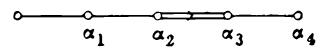
\includegraphics[keepaspectratio]{images/part002_560ef793.jpg}}

\begin{enumerate}
\def\labelenumi{(\Alph{enumi})}
\setcounter{enumi}{21}
\tightlist
\item
  \(R^{\prime}\) 是向量集 \(\pm2\varepsilon_{i},\pm\varepsilon_{i}\pm\varepsilon_{j},\pm\varepsilon_{1}\pm\varepsilon_{2}\pm\varepsilon_{3}\pm\varepsilon_{4}.\)
\end{enumerate}

\[
  \Phi_ {\mathrm{R}} (x, y) = \frac {(x | y)}{18}, \quad \gamma (\mathrm{R}) = 2. 3 ^ {4}.
\]

\begin{enumerate}
\def\labelenumi{(\Roman{enumi})}
\setcounter{enumi}{5}
\tightlist
\item
  基本权：
\end{enumerate}

\[
\omega_ {1} = \varepsilon_ {1} + \varepsilon_ {2} = 2 \alpha_ {1} + 3 \alpha_ {2} + 4 \alpha_ {3} + 2 \alpha_ {4}
\]

\[
\omega_ {2} = 2 \varepsilon_ {1} + \varepsilon_ {2} + \varepsilon_ {3} = 3 \alpha_ {1} + 6 \alpha_ {2} + 8 \alpha_ {3} + 4 \alpha_ {4}
\]

\[
\omega_ {3} = \frac {1}{2} (3 \varepsilon_ {1} + \varepsilon_ {2} + \varepsilon_ {3} + \varepsilon_ {4}) = 2 \alpha_ {1} + 4 \alpha_ {2} + 6 \alpha_ {3} + 3 \alpha_ {4}
\]

\[
\omega_ {4} = \varepsilon_ {1} = \alpha_ {1} + 2 \alpha_ {2} + 3 \alpha_ {3} + 2 \alpha_ {4}.
\]

\begin{enumerate}
\def\labelenumi{(\Roman{enumi})}
\setcounter{enumi}{6}
\tightlist
\item
  正根之和：
\end{enumerate}

\[
2 \rho = 11 \varepsilon_ {1} + 5 \varepsilon_ {2} + 3 \varepsilon_ {3} + \varepsilon_ {4} = 16 \alpha_ {1} + 30 \alpha_ {2} + 42 \alpha_ {3} + 22 \alpha_ {4}.
\]

\begin{enumerate}
\def\labelenumi{(\Roman{enumi})}
\setcounter{enumi}{7}
\tightlist
\item
  \(\mathrm{Q}(\mathrm{R}) = \bigoplus_{i=1}^{4} \mathbf{Z} \varepsilon_i + \mathbf{Z}\left(\frac{1}{2} \sum_{i=1}^{4} \varepsilon_i\right)\) .
\end{enumerate}

\(P(R) = Q(R).\)

连接指标：1。

\begin{enumerate}
\def\labelenumi{(\Roman{enumi})}
\setcounter{enumi}{8}
\item
  指数：1, 5, 7, 11。
\item
  以及（XI）A(R) = W(R)，\(w_{0} = -1\) 。
\item
  Cartan 矩阵：
\end{enumerate}

\[
\left( \begin{array}{c c c c} 2 & - 1 & 0 & 0 \\ - 1 & 2 & - 2 & 0 \\ 0 & - 1 & 2 & - 1 \\ 0 & 0 & - 1 & 2 \end{array} \right)
\]

